\documentclass[11pt, a4paper]{article}
\usepackage{pdfpages}
\usepackage{parallel}
\usepackage[T2A]{fontenc}
\usepackage{ucs}
\usepackage[utf8x]{inputenc}
\usepackage[polish,english,russian]{babel}
\usepackage{hyperref}
\usepackage{rotating}
\usepackage[inner=2cm,top=1.8cm,outer=2cm,bottom=2.3cm,nohead]{geometry}
\usepackage{listings}
\usepackage{graphicx}
\usepackage{wrapfig}
\usepackage{longtable}
\usepackage{indentfirst}
\usepackage{array}
\usepackage{tikzsymbols}
\usepackage{soul}
\usepackage[ruled,vlined]{algorithm2e}
%\counterwithout{figure}{section} 

\usepackage{url}
\makeatletter
\g@addto@macro{\UrlBreaks}{\UrlOrds}
\makeatother

\newcolumntype{P}[1]{>{\raggedright\arraybackslash}p{#1}}
\frenchspacing
\usepackage{fixltx2e} %text sub- and superscripts
\usepackage{icomma} % коскі ў матэматычным рэжыме
\PreloadUnicodePage{4}

\newcommand{\longpage}{\enlargethispage{\baselineskip}}
\newcommand{\shortpage}{\enlargethispage{-\baselineskip}}

\def\switchlang#1{\expandafter\csname switchlang#1\endcsname}
\def\switchlangbe{
\let\saverefname=\refname%
\def\refname{Літаратура}%
\def\figurename{Іл.}%
}
\def\switchlangen{
\let\saverefname=\refname%
\def\refname{References}%
\def\figurename{Fig.}%
}
\def\switchlangru{
\let\saverefname=\refname%
\let\savefigurename=\figurename%
\def\refname{Литература}%
\def\figurename{Рис.}%
}

\hyphenation{admi-ni-stra-tive}
\hyphenation{ex-pe-ri-ence}
\hyphenation{fle-xi-bi-li-ty}
\hyphenation{Py-thon}
\hyphenation{ma-the-ma-ti-cal}
\hyphenation{re-ported}
\hyphenation{imp-le-menta-tions}
\hyphenation{pro-vides}
\hyphenation{en-gi-neering}
\hyphenation{com-pa-ti-bi-li-ty}
\hyphenation{im-pos-sible}
\hyphenation{desk-top}
\hyphenation{elec-tro-nic}
\hyphenation{com-pa-ny}
\hyphenation{de-ve-lop-ment}
\hyphenation{de-ve-loping}
\hyphenation{de-ve-lop}
\hyphenation{da-ta-ba-se}
\hyphenation{plat-forms}
\hyphenation{or-ga-ni-za-tion}
\hyphenation{pro-gramming}
\hyphenation{in-stru-ments}
\hyphenation{Li-nux}
\hyphenation{sour-ce}
\hyphenation{en-vi-ron-ment}
\hyphenation{Te-le-pathy}
\hyphenation{Li-nux-ov-ka}
\hyphenation{Open-BSD}
\hyphenation{Free-BSD}
\hyphenation{men-ti-on-ed}
\hyphenation{app-li-ca-tion}

\def\progref!#1!{\texttt{#1}}
\renewcommand{\arraystretch}{2} %Іначай формулы ў матрыцы зліпаюцца з лініямі
\usepackage{array}

\def\interview #1 (#2), #3, #4, #5\par{

\section[#1, #3, #4]{#1 -- #3, #4}
\def\qname{LVEE}
\def\aname{#1}
\def\q ##1\par{{\noindent \bf \qname: ##1 }\par}
\def\a{{\noindent \bf \aname: } \def\qname{L}\def\aname{#2}}
}

\def\interview* #1 (#2), #3, #4, #5\par{

\section*{#1\\{\small\rm #3, #4. #5}}
\ifx\ParallelWhichBox\undefined%
    \addcontentsline{toc}{section}{#1, #3, #4}%
\else%
\ifnum\ParallelWhichBox=0%
    \addcontentsline{toc}{section}{#1, #3, #4}%
\fi\fi%

\def\qname{LVEE}
\def\aname{#1}
\def\q ##1\par{{\noindent \bf \qname: ##1 }\par}
\def\a{{\noindent \bf \aname: } \def\qname{L}\def\aname{#2}}
}

\newcommand{\interviewfooter}[1]{
\vskip 1em
\noindent \textit{#1}
}

\switchlang{en}
\begin{document}

\title{1996 "--- Q500 mouse}
\date{}
\maketitle
\selectlanguage{english}
The Q500 mouse (fig. \ref{fig:q500mousePic}) was produced in South Korea and was (along with the Hi-Bon Optical laser mouse LMOX-2) one of two unusual optical mice with light guides, developed in 1996 by iO TEK. The Q500 mouse probably has the cheapest optical mouse design ever invented.

\begin{figure}[h]
    \centering
    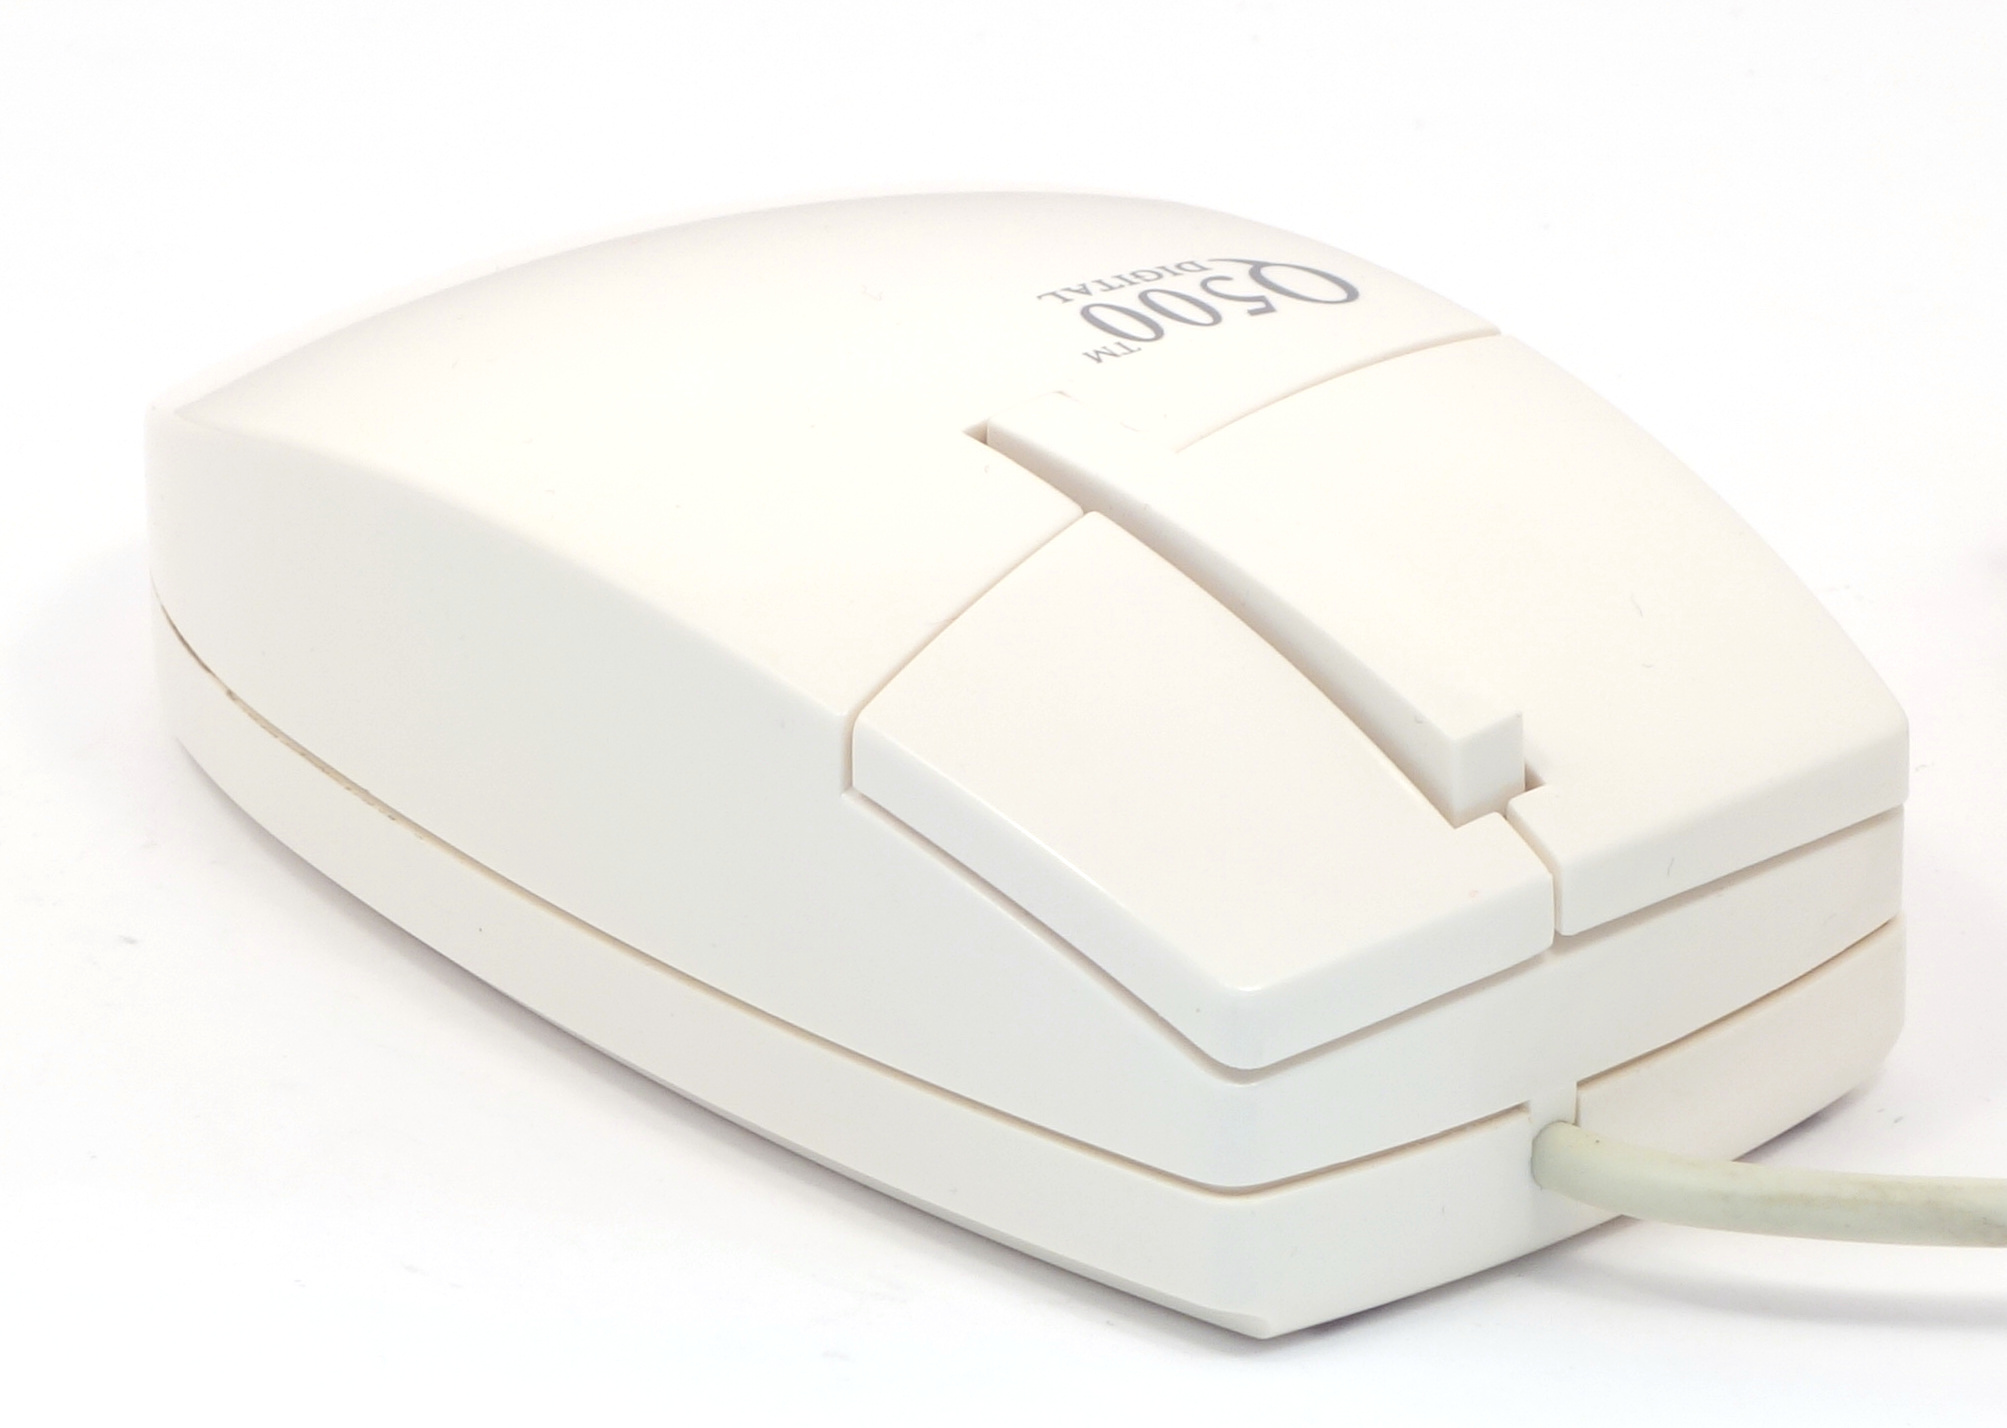
\includegraphics[scale=0.5]{1996_q500_mouse/pic_30.jpg}
    \caption{Q500 mouse}
    \label{fig:q500mousePic}
\end{figure}

As with the vast majority of early optical mice, this mousepad requires a reflective mesh pad (fig. \ref{fig:q500mousePad}). Unlike the Mouse Systems metal pads with a grating of vertical and horizontal lines for two different wavelengths, here you can see a light surface with dark lines (fig. \ref{fig:q500mousePad}). As you can see, two blocks are used (a block of horizontal lines and a block of vertical lines), each of which occupies half of the pad.



\begin{figure}[h]
    \centering
    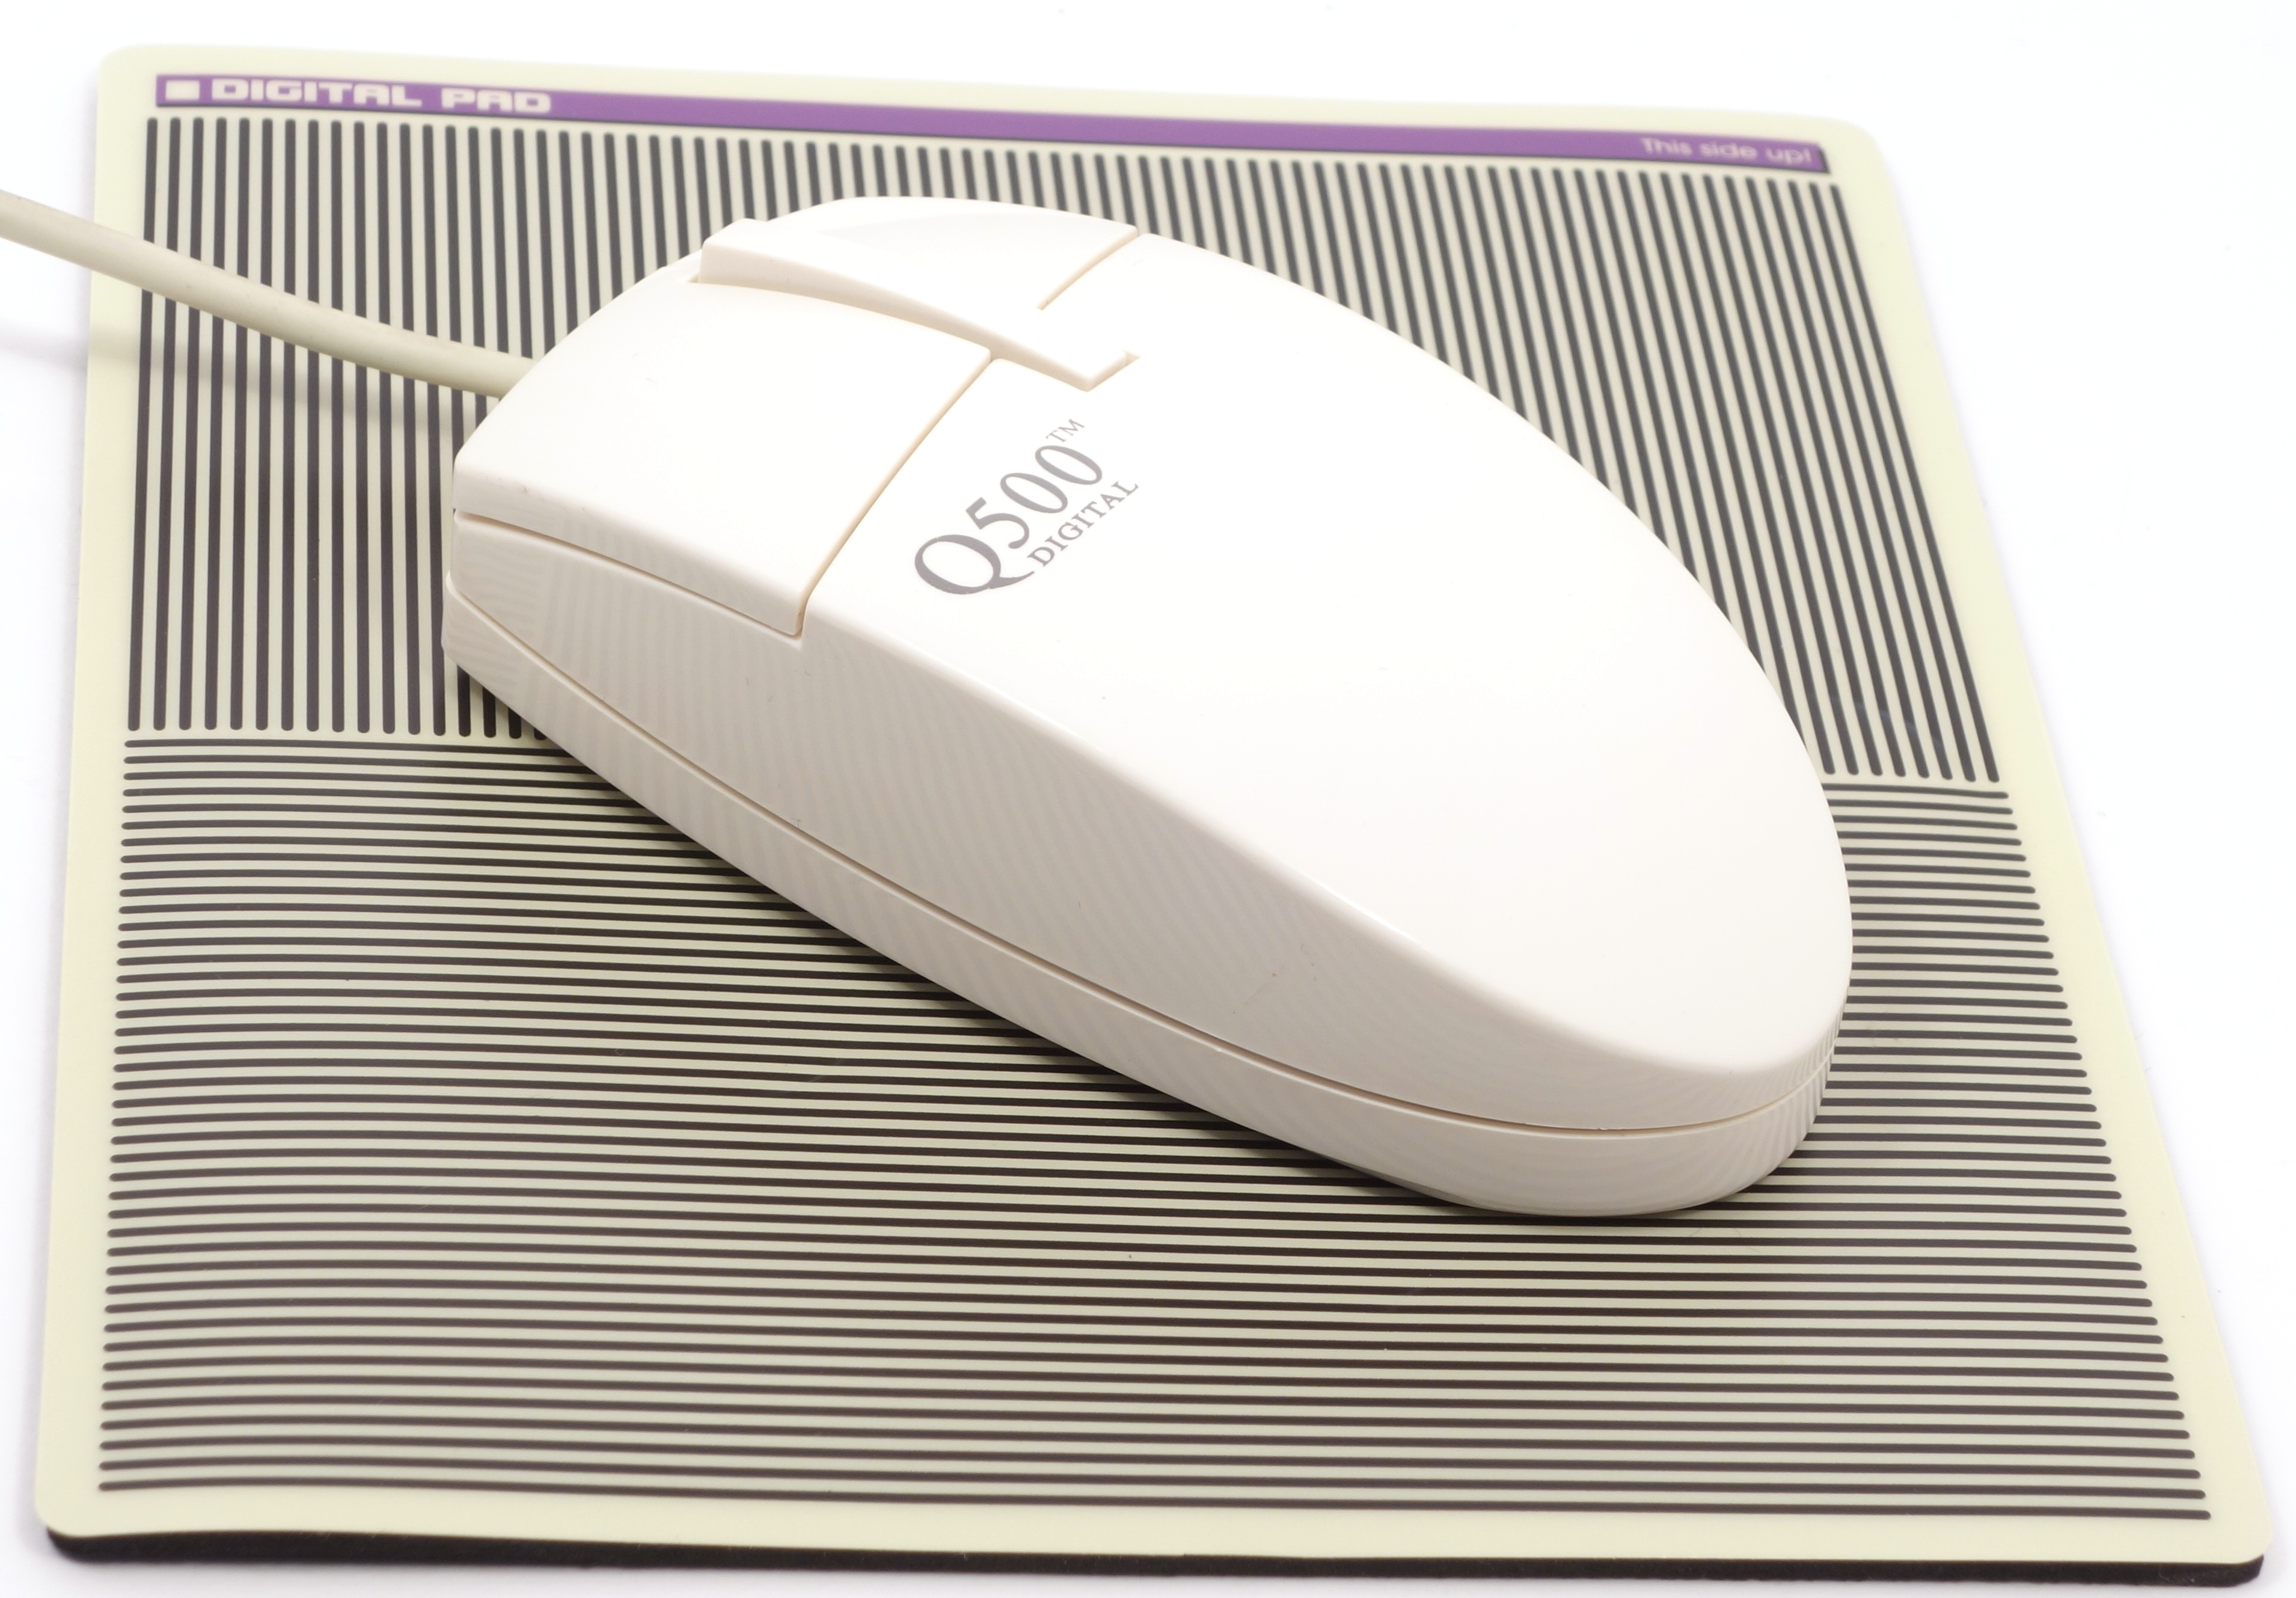
\includegraphics[scale=0.4]{1996_q500_mouse/pad_30.jpg}
    \caption{Q500 mouse on its pad}
    \label{fig:q500mousePad}
\end{figure}

The small size of the pad is explained by the fact that each of the two mouse sensors corresponds to its own block of lines.
The two mouse sensors are located in the body of the mouse as far apart as possible (fig. \ref{fig:q500mouseTopBottom}) so that they cannot lose their respective areas, even if you move the mouse to the very edge of the mousepad. Therefore, increasing the pad would require a similar increase in the size of the mouse.

The design of the Q500 is essentially a modification of a standard optomechanical mouse based on a pair of rotary encoders: in the case of the Q500, the slots on the encoder disks are turned into a block of lines on the pad (that is, the rotary encoders are replaced by linear ones). This similarity makes it possible to use any opto-mechanical mouse controller chip in the Q500, simplifying the choice of element base. \cite{yq}.

\begin{figure}[h]
    \centering
    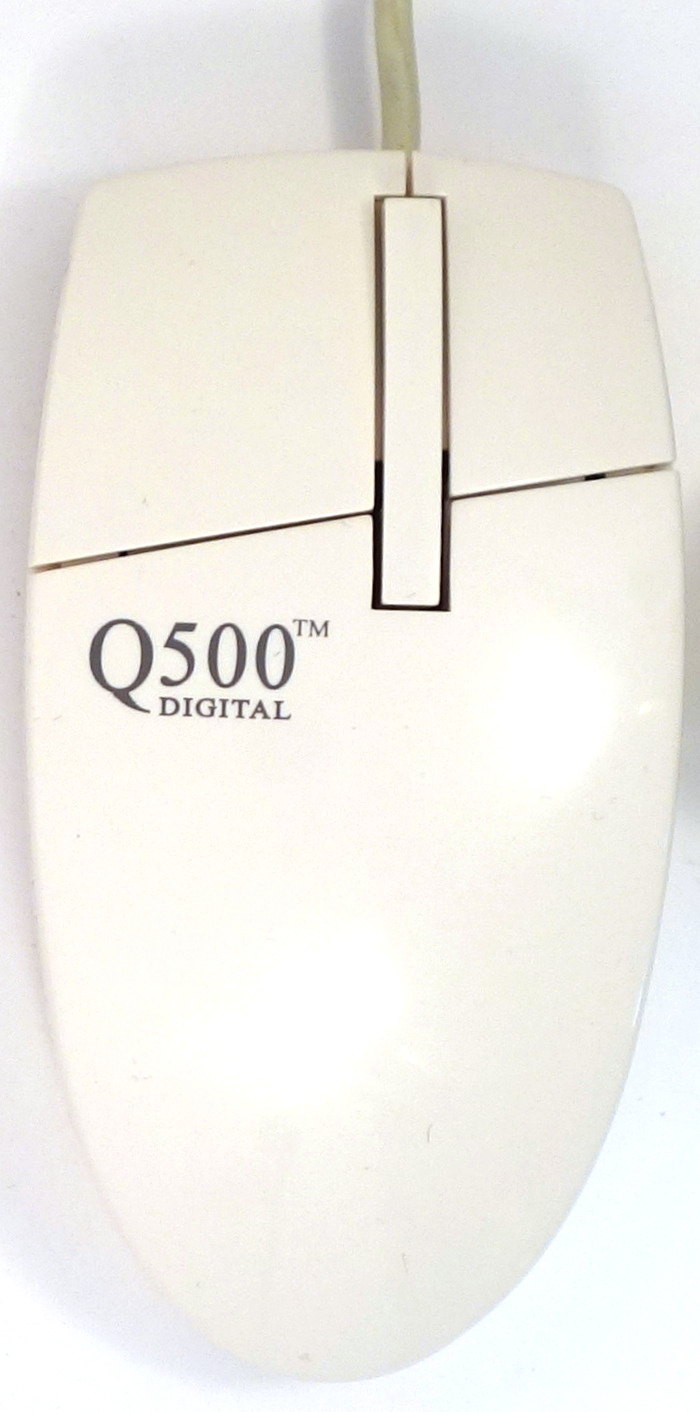
\includegraphics[scale=0.5]{1996_q500_mouse/top_30.jpg}
    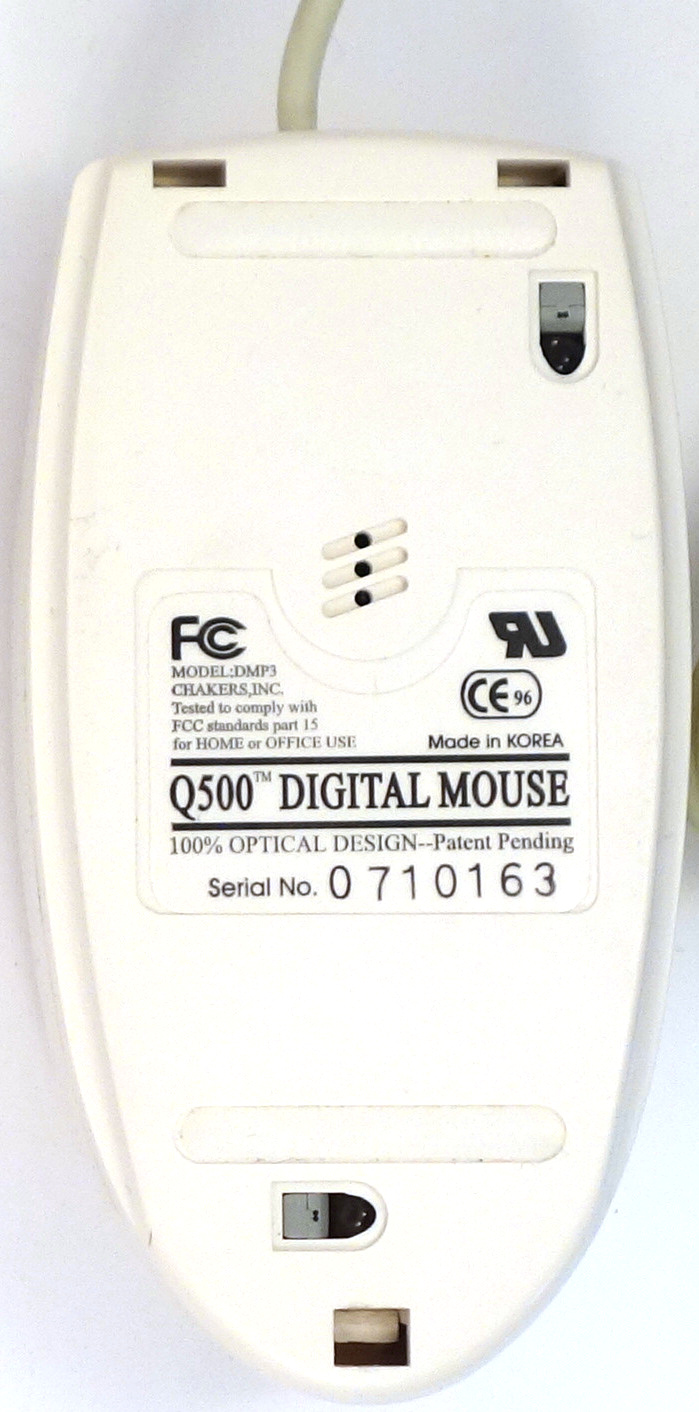
\includegraphics[scale=0.5]{1996_q500_mouse/bottom_30.jpg}
    \caption{Q500 mouse, top and bottom views}
    \label{fig:q500mouseTopBottom}
\end{figure}

The size and shape of the mouse is typical cursor controller device of the 90s (fig. \ref{fig:q500mouseSize}).

\begin{figure}[h]
    \centering
    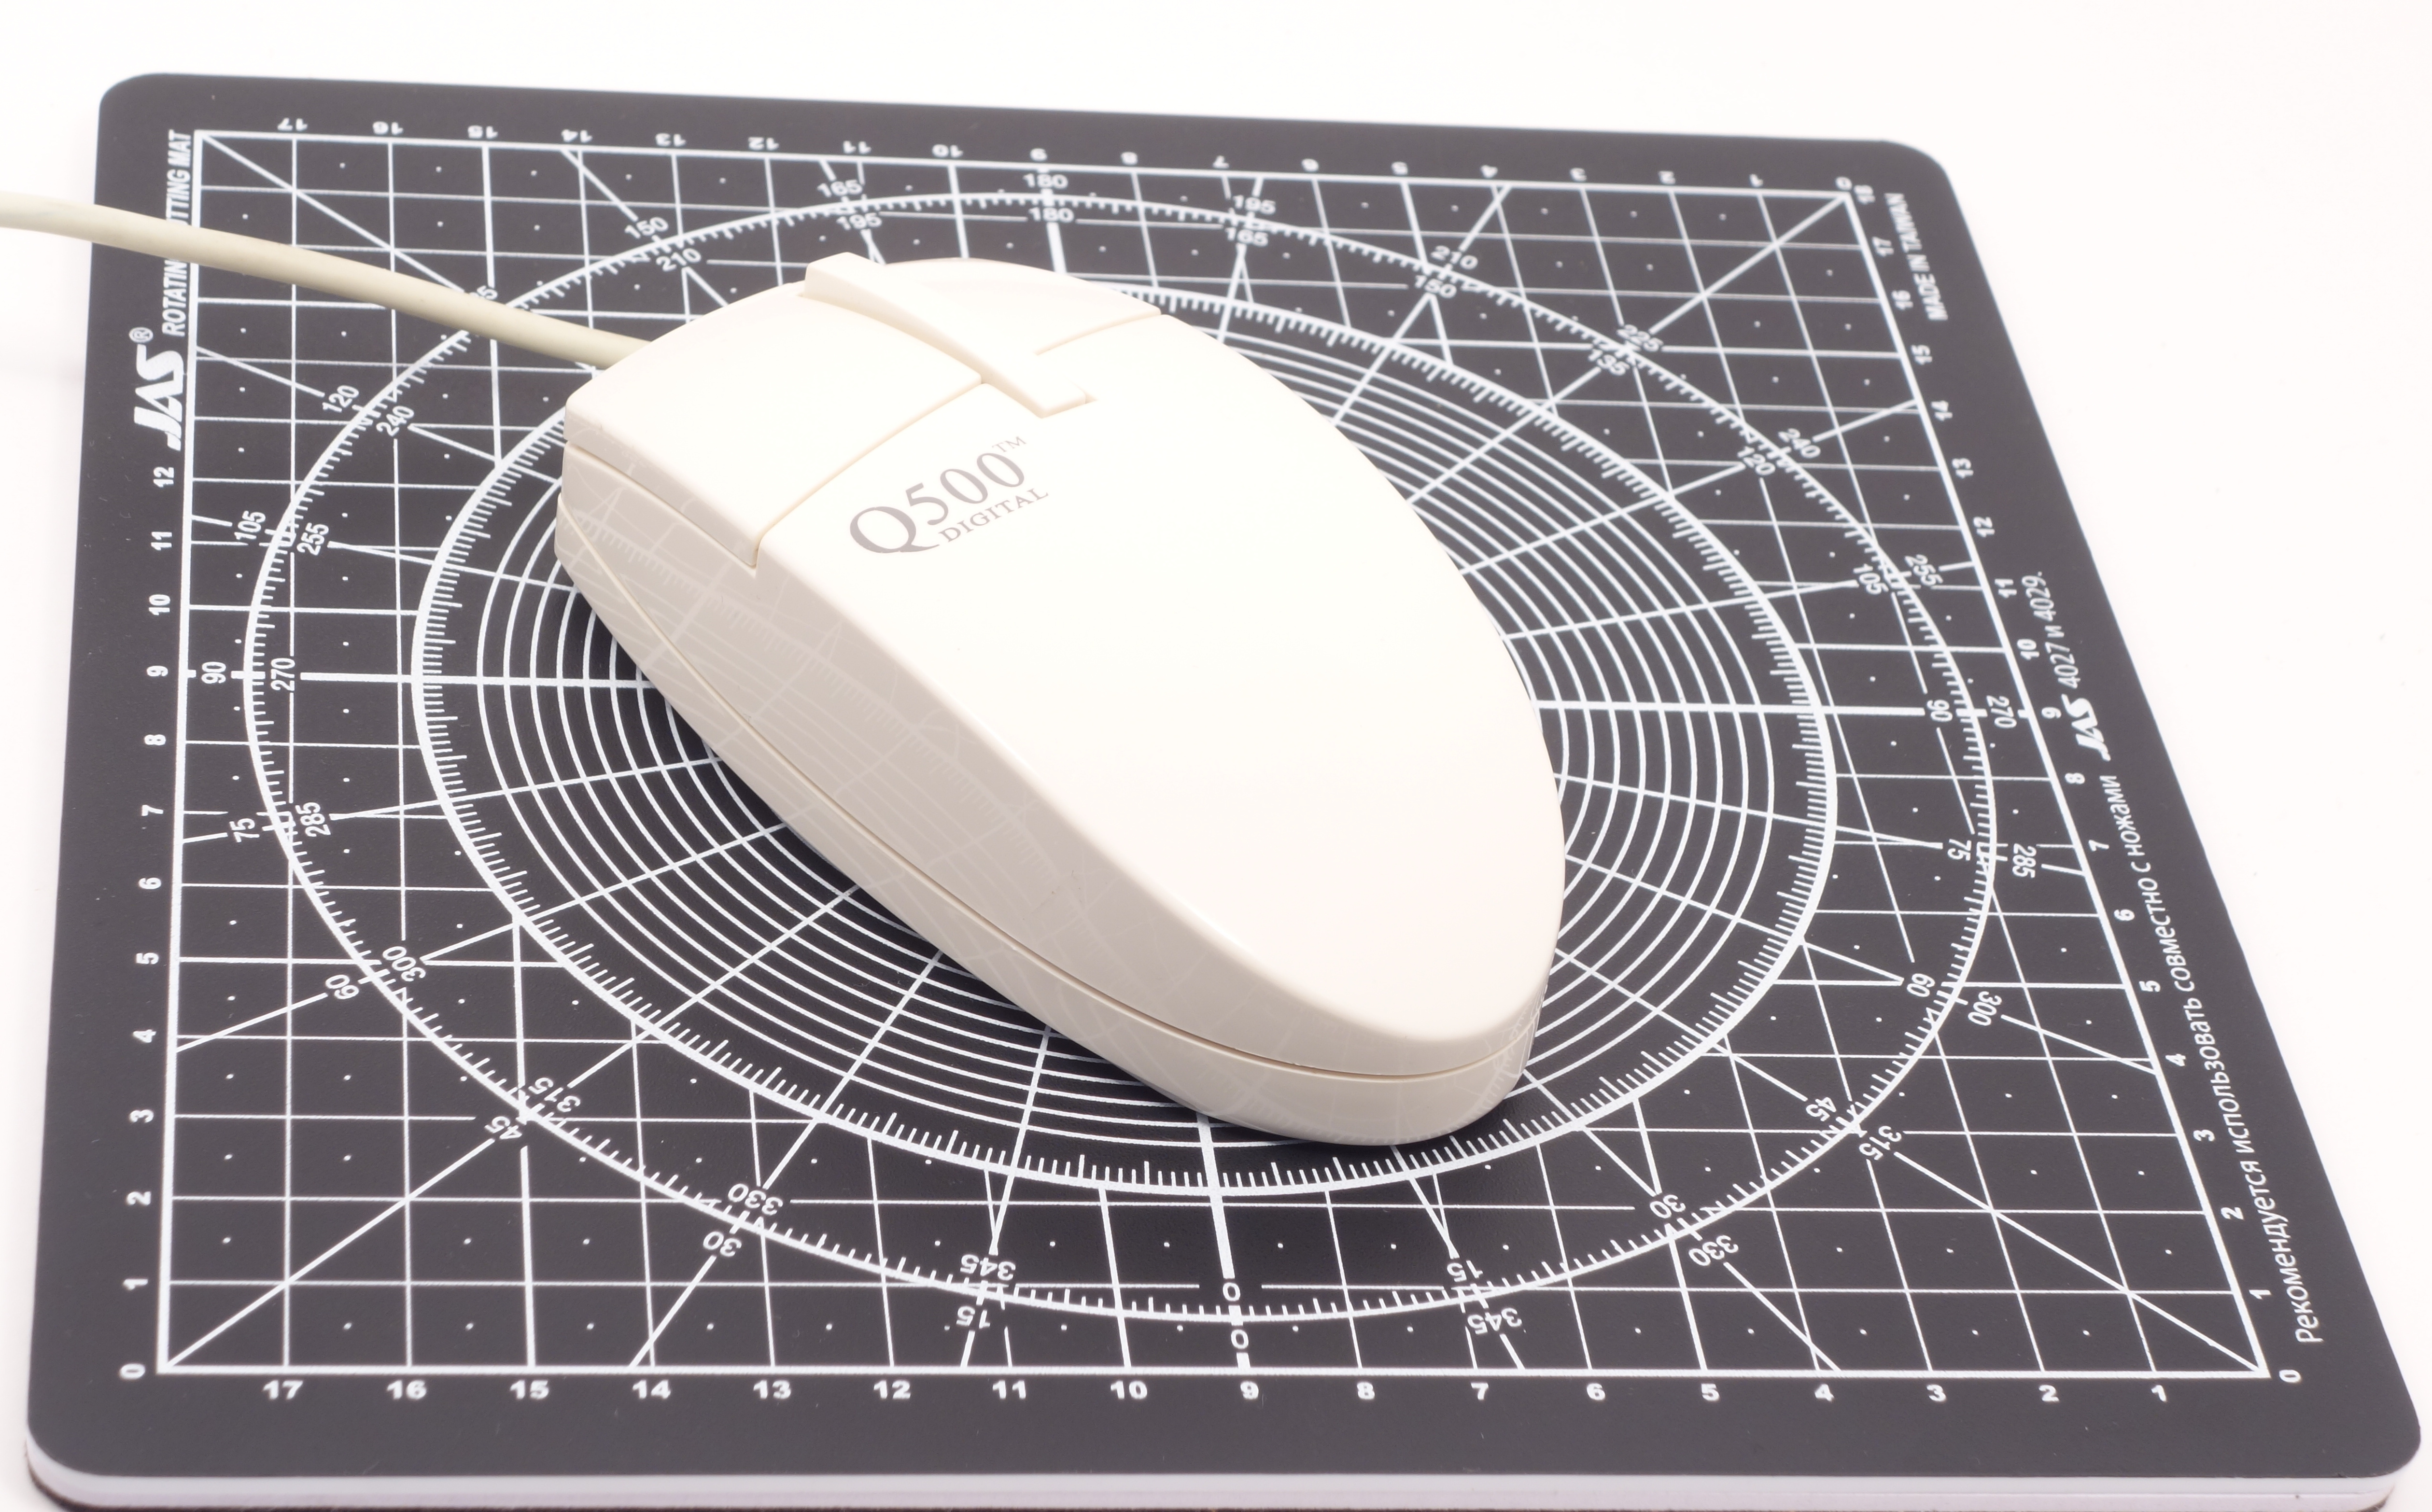
\includegraphics[scale=0.25]{1996_q500_mouse/size.jpg}
    \caption{Q500 mouse on a graduated pad with a grid step of 1~cm}
    \label{fig:q500mouseSize}
\end{figure}

The mouse has rather comfortable left and right buttons (fig. \ref{fig:q500mouseHand}), as well as a third narrow button, the shape of which suggests that it is hardly intended for frequent clicks.

\begin{figure}[h]
    \centering
    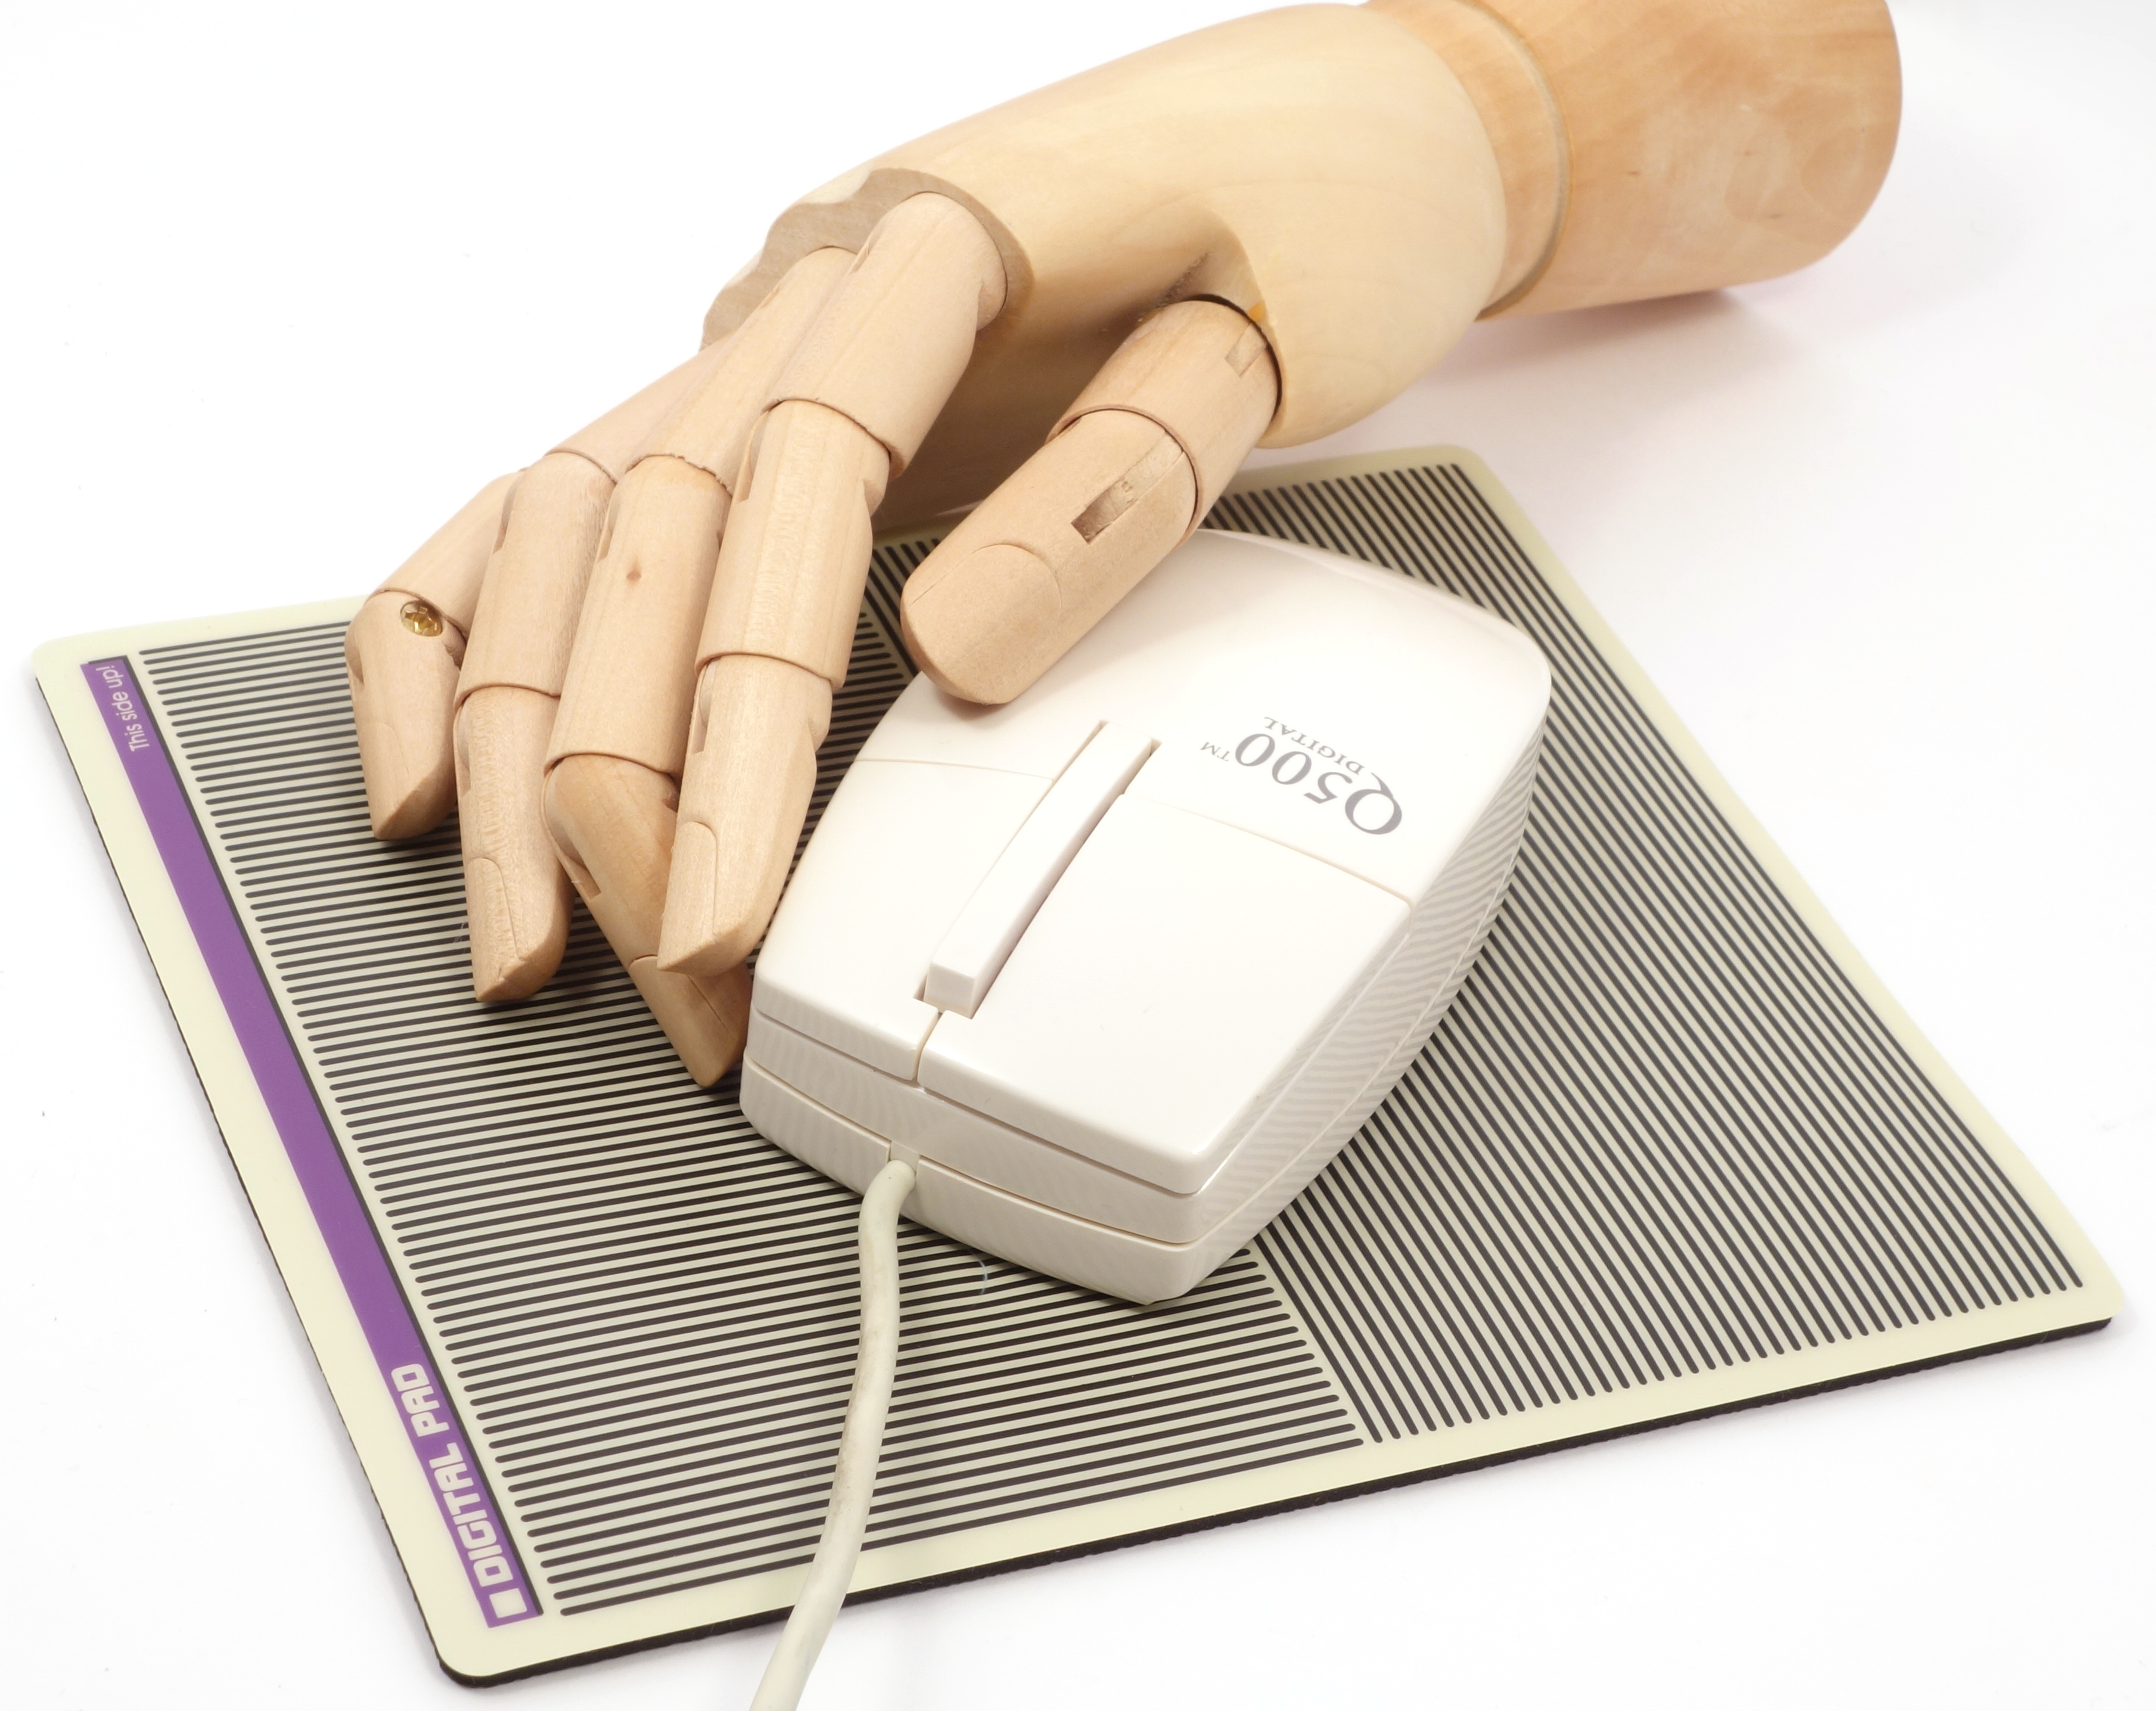
\includegraphics[scale=0.4]{1996_q500_mouse/hand_30.jpg}
    \caption{Q500 with a human hand model}
    \label{fig:q500mouseHand}
\end{figure}


The internals are shown in fig. \ref{fig:q500mouseInside}.
The halves of the case are connected by latches, without screws. A monolithic block in the center, where the light guides enter, hides two photodiodes. Unlike Mouse Systems mice that use separate sensors for each axis, the Q500 design is further reduced in cost by cycling the LEDs so that the photodiodes are first sampled horizontally and then vertically \cite{yq}.

\begin{figure}[h]
    \centering
    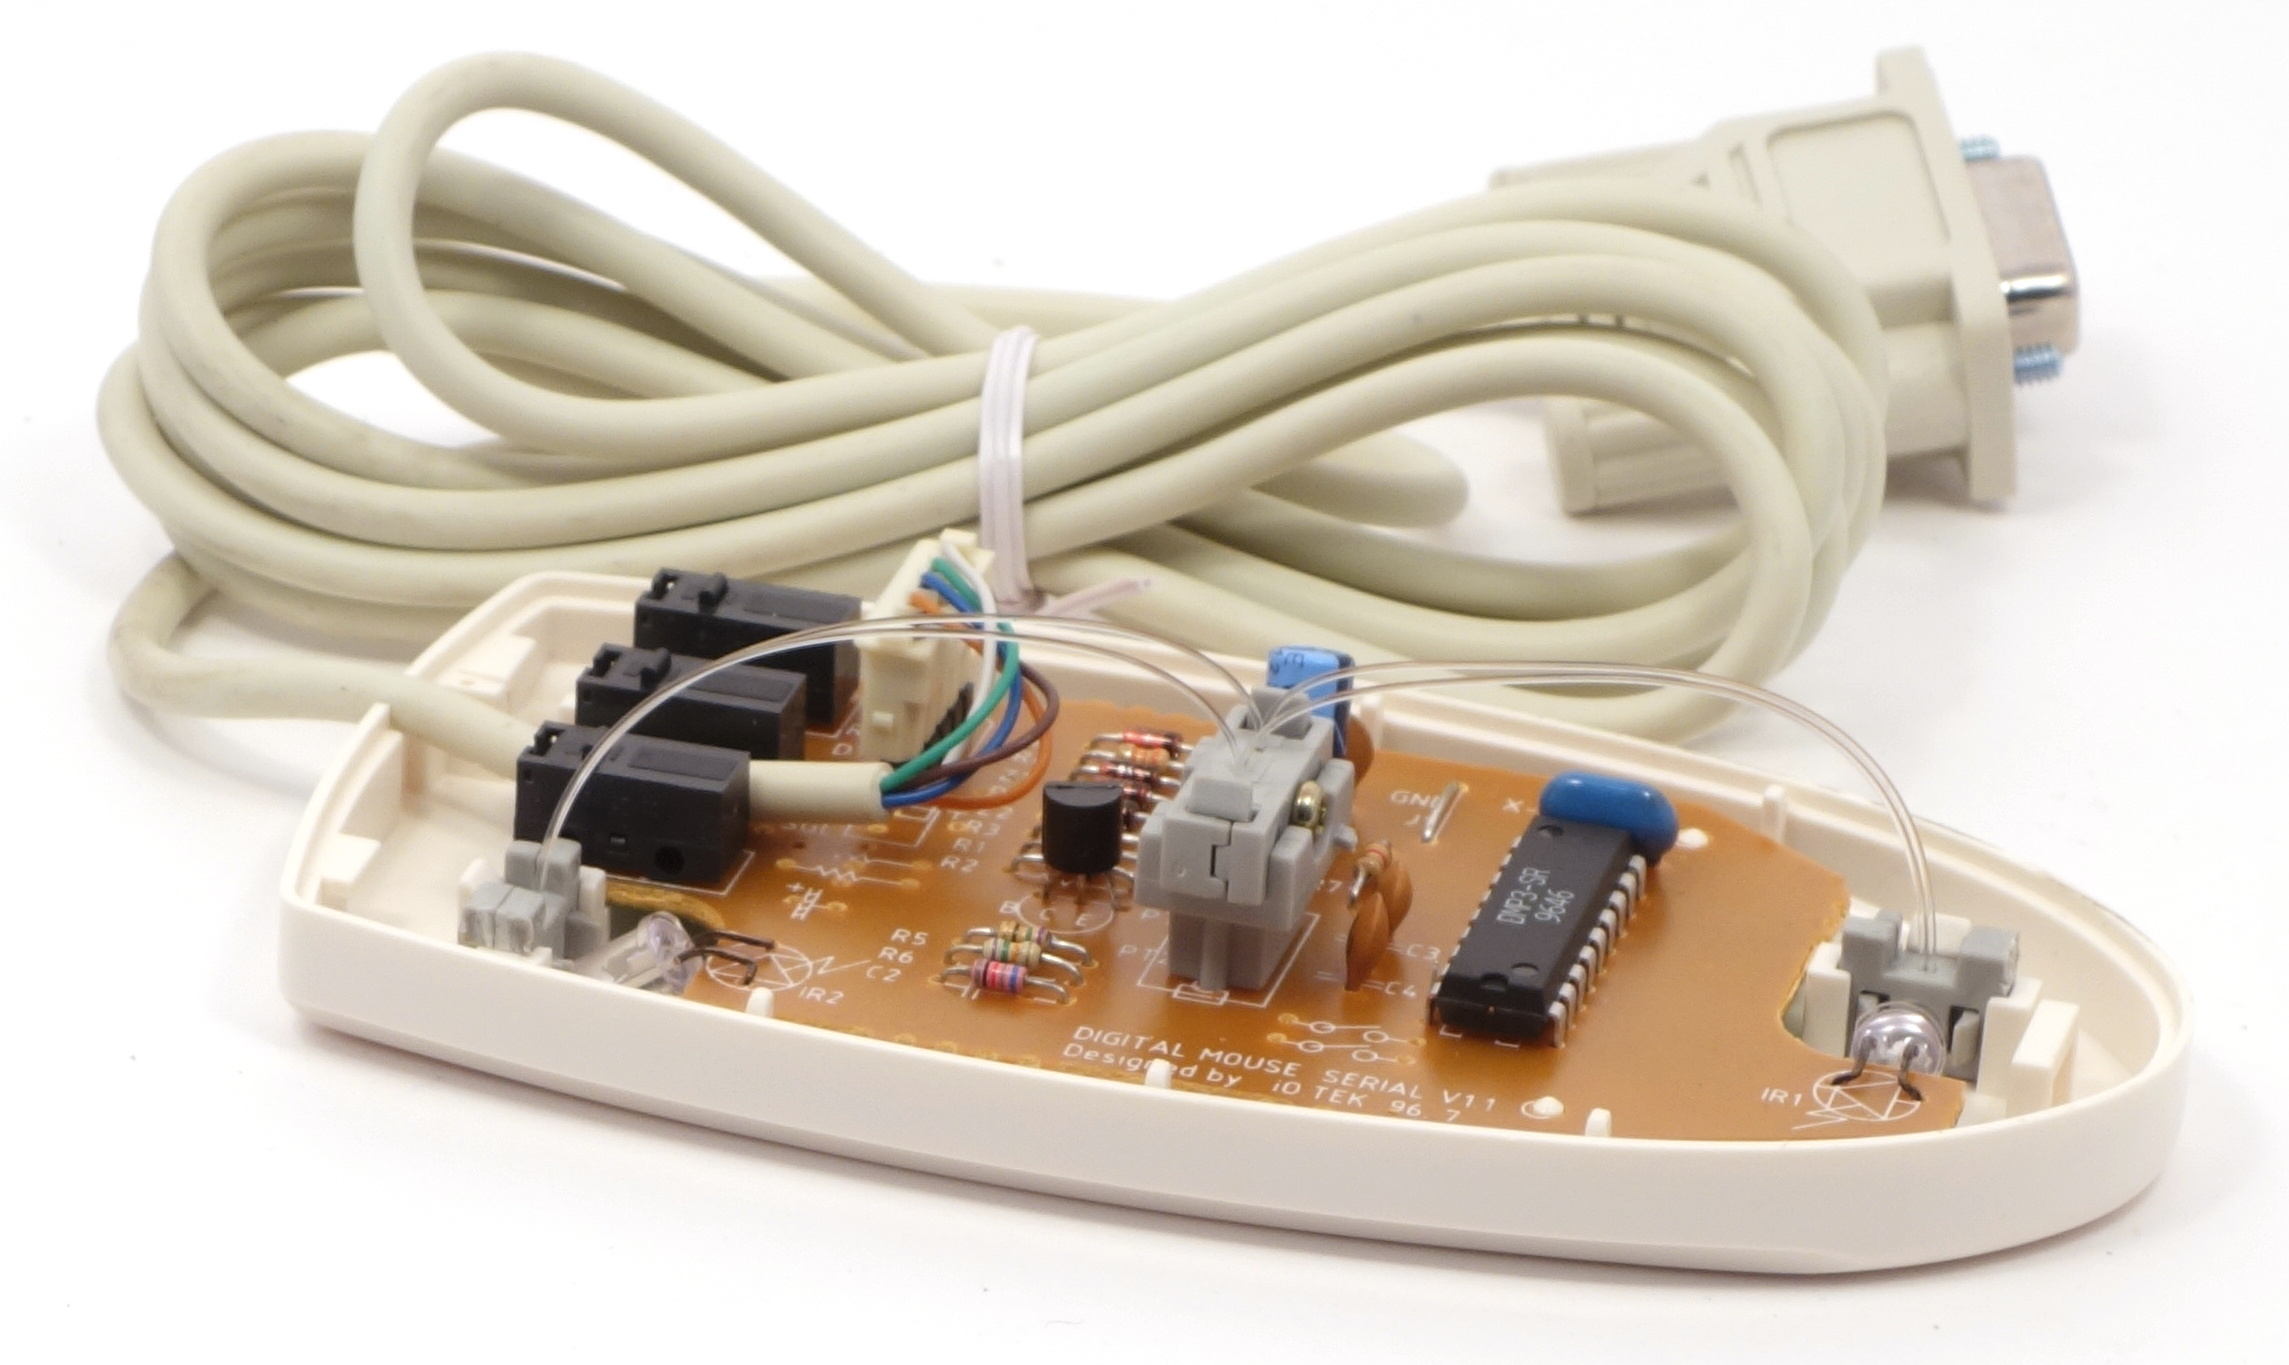
\includegraphics[scale=0.8]{1996_q500_mouse/inside_30.jpg}
    \caption{Q500 mouse disassembled}
    \label{fig:q500mouseInside}
\end{figure}

The text on the PCB shows that this mouse was, like the Hi-Bon Optical laser mouse, developed under contract by iO TEK in 1996.

At the same time, according to the video review given in \cite{yq}, in practice the mouse moves the cursor only slightly more roughly than a regular mouse. The only real problem is that if the pad cannot be rotated relative to the mouse (not even slightly). Also, if the edge of the mouse (and, accordingly, one of the sensors) goes beyond the pad, the mouse loses the ability to register movements along the corresponding axis.

\begin{thebibliography}{9}
\bibitem {yq} Q500, The Weirdest Optical Mouse \url{https://www.youtube.com/watch?v=Cd6lxwjX2Bk}
\end{thebibliography}
\end{document}
